%%This is a very basic article template.
%%There is just one section and two subsections.
\documentclass[a4paper,landscape,10pt]{article}
%\DeclareMathSizes{10}{8}{8}{7}   % For size 10 text
%\DeclareMathSizes{11}{8}{8}{7}   % For size 11 text
%\everymath=\expandafter{\the\everymath\displaystyle}


\usepackage[margin=0.5cm]{geometry}
\usepackage{multicol}

\usepackage{amsfonts}
\usepackage{amsopn}
\usepackage{amsmath}

\usepackage{graphicx}
\graphicspath{{./resources/}}

% change style of items
\newlength{\wideitemsep}
\setlength{\wideitemsep}{.5\itemsep}
\addtolength{\wideitemsep}{-7pt}
\let\olditem\item
\renewcommand{\item}{\setlength{\itemsep}{\wideitemsep}\olditem}

\usepackage{enumitem}
\setlist[itemize]{leftmargin=*}
\setlist[description]{leftmargin=*}
\setlist[enumerate]{leftmargin=*}

\usepackage{sectsty}
\sectionfont{\large}
\subsectionfont{\small}
\subsectionfont{\small}

\usepackage{algpseudocode}
\usepackage{algorithmicx}

%reset itemseparator for algorithms
\usepackage{etoolbox}
\makeatletter
\expandafter\patchcmd\csname\string\algorithmic\endcsname{\itemsep\z@}{\wideitemsep=0.5\itemsep}{}{}
\makeatother

\newcommand{\R}[0]
{
    \mathbb{R}%
}

\renewcommand*{\O}[0] {\ensuremath{\mathcal{O}}}

\DeclareMathOperator*{\argmin}{arg\,min}
\DeclareMathOperator*{\argmax}{arg\,max}

\title{Computational Intelligence Lab 2013}
\author{Dominic Langenegger}

\begin{document}
\begin{multicols}{4}

%vertical spaces of equations
\abovedisplayskip=0pt
\belowdisplayskip=5pt
\abovedisplayshortskip=0pt
\belowdisplayshortskip=5pt


%\maketitle


\section{Dimensionality Reduction}
\subsection{Principal Component Analysis}
Minimizing error $\|x_n - \tilde{x}_n\|$ and maximizing
variance and therefore revealing interesting information.

Covariance of the data with mean $\bar{x}$:

\[
    \Sigma = \frac{1}{N} \sum_{n=1}^N (x_n - \bar{x}) (x_n - \bar{x})^\top
\]

With the mean of the projected data being $u_i^\top \bar{x}$ we maximize
the variance $u_i^\top \Sigma u_1$ such that $\|u_i\|_2 = 1$.

Using the Lagrangian of this optimization problem and setting the derivative to
zero we get:

\[
    \Sigma u_1 = \lambda_1 u_1
\]

Eigendecomposition Problem $\Sigma = U \Lambda U^\top$: To maximize the variance
we simply choose the eigenvector with the larges associated eigenvalue. This is
called the first ($n^{th}$) {\bf principal direction}.

For $K \leq D$ dimensional projection space we choose $K$ eigenvectors $\{u_1,
\ldots, u_K\}$ with largest associated eigenvalues $\{\lambda_1, \ldots,
\lambda_K\}$. We call these eigenvectors the {\bf principal components} in a PCA
of $A$.

\subsubsection{Matrix Viewpoint}

When computing the projection of $\bar{X}$ on $U_k = [u_1, \ldots, u_K]$
(eigenvectors with the $K$ highest eigenvalues of covariance matrix $\Sigma$)
we get:

\begin{align*}
    \bar{Z}_K       &= U_K^\top \cdot \bar{X} \quad &\text{(project on $U_k$)}\\
    \tilde{\bar{X}} &= U_K \cdot \bar{Z}_K    \quad &\text{(original basis)}\\
    \tilde{X}       &= \tilde{\bar{X}} + M    \quad &\text{(re-add mean)}
\end{align*}

\subsection{Singular Value Decomposition (SVD)}
Every rectangular matrix has an SVD decomposition into a set of three matrix
factors:

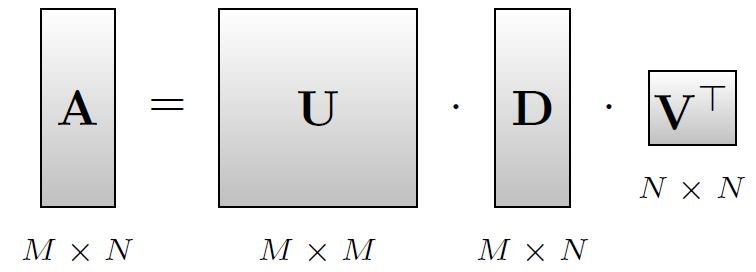
\includegraphics[width=0.9\linewidth]{svd-dimensions}

With $U, V^\top$ orthogonal and $D$ diagonal. The non-zero elements in $D$ on
the diagonal are called the {\bf singular values} and are equal to the square
roots of the eigenvalues of $AA^\top$ and $A^\top A$. The corresponding
eigenvectors are the columns of $U$ and the rows of $V^\top$, respectively.

The first $r$ columns of $U$ are called the {\bf left singular vectors} and form
an orthogonal basis for the space spanned by the columns of the original matrix
$A$. Similar with rows of $V^\top$ which form row space of $A$.

In Collaborative Filtering (Movie Rating):
\begin{align*}
    U: \quad &\text{User-to-concept affinity} \\
    V: \quad &\text{Movie-to-concept affinity} \\
    D: \quad &\text{Strength of concept}
\end{align*}

\subsubsection{Closest Rank-$k$ Matrix}
With $A_k = \sum_{i=1}^k d_i u_i v_i^\top$ being a matrix with rank $k < r =
rank(A)$ we have the closest rank-$k$ approximation to $A$ in the Euclidean
matrix norm sense. 

Magnitudes of the nonzero singular values provide a measure of approximation to
$A_k$: $\|A - A_k\|_2 = d_{k+1}$.
If square matrix $\rightarrow$ spectral norm: $\|A\|_2 = \sigma_{max}(A)$

\subsubsection{Computing the SVD}
Given a matrix $A \in \R^{M \times N}$ (assume $N < M$)
\begin{enumerate}
    \item Eigenvalue-decomposition of $A^\top A$. Fill roots of eigenvalues into
    $D$.
    \item Compute the eigenvectors of $A^\top A$. Place them (in the right
    order) along the columns of $V$. (rows of $V^\top$)
    \item Compute the matrix $U$ as $AVD^{-1}$. ($D_{ii}^{-1} =
    \frac{1}{D_{ii}}$)
\end{enumerate}

If $S$ is a real and symmetric matrix ($S = S^\top$) then $S = UDU^\top$.


\section{Clustering}
Assign data points to cluster and minimize the following cost function:

\[
    J(U, Z) = \|X - UZ\|_F^2 = \sum_{n=1}^{N}\sum_{k=1}^K z_{k,n} \|x_n -
    u_k\|_2^2
\]

Where $X = [x_1 \cdots x_N] \in \R^{D \times N}$, $U = [u_1 \cdots u_K] \in
\R^{D \times K}$. We call the $u_k$ the {\bf centroids} and $z_n$ the
assignments of data points to clusters.

\subsection{K-Means}
{\bf Hard assignment}: $Z \in \{0,1\}^{K \times N}$ with $\sum_k z_{k,n} = 1 \;
\forall n$.

\begin{enumerate}
    \item Initialize centroids
    \item Assign data points to clusters. \\
            $k^*(x_n)$ index with the minimal distance:
            \begin{equation*}
            \begin{split}
                k^*(x_n) = \argmin_{k} \big\{ &\|x_n - u_1 \|_2^2 \quad \forall
                i \big\}
            \end{split}
            \end{equation*}
    \item Update Cluster Centroids: \\
            Compute the mean/centroid of a cluster:
            \[
                u_k = \frac{\sum_{n=1}^N z_{k,n}x_n}{\sum_{n=1}^N z_{k,n}} \quad
                \forall k, k \in \{1, \ldots, K \}
            \]
\end{enumerate}
Iterate until ($\O(KN)$ per iteration):
\begin{equation*}
\begin{split}
    \| u_k^{(t)} - u_k^{(t-1)} \|_2^2 < \epsilon \quad &\forall k \text{ with }
    (0 < \epsilon \ll 1) \\
   \text{or until } &t = t_{finish}
\end{split}
\end{equation*}

\begin{itemize}
    \item K-means convergence is guaranteed
    \item Non-convex objective, local minima, sensitive to initializations.
    $\rightarrow$ restarts.
\end{itemize}

\subsubsection{Clustering Stability}
\begin{enumerate}
    \item Generate pertrubed versions of the set
    \item Apply algorithm on all versions
    \item Pair-wise distance between clusterings
    \item Compute the {\bf instability} as the mean distance between all
    clusterings
\end{enumerate}

Repeat for different numbers of clusters and choose the one that
minimizes the instability.

The distance between two clusterings $C$ and $C'$ can be calculated as follows:
\begin{equation*}
    d = \min_\pi \| Z - \pi(Z') \|_0
\end{equation*}
where $\pi(Z')$ is one of the possible row permutations of $Z'$ and $\|Z\|_0$
denotes the cardinality of $Z$.

\subsection{Mixture Models (Soft Clustering)}
Relax the hard constraint given by $Z \in \{0,1\}^{K \times N}$ with $\sum_k
z_{k,n} = 1 \; \forall n$ from $k$-means with a soft one:
$z_{k,n} \in [0,1] \text{ with } \sum_{k=1}^{K} z_{k,n} = 1 \quad \forall n$.
Definition:

\begin{align*}
    p(x) = \sum_{k=1}^K \pi_k p(x | \Theta_k)
\end{align*}

\subsubsection{Gaussian Mixture Models}

Independent identically distributed points. Use {\bf Expectation-Maximation} to
find maximum likelihood solutions for models with latent variables. Find
parameters $\pi, \mu, \Sigma$.

\begin{align*}
    \ln\;p(X &| \pi, \mu, \Sigma) = \sum_{n=1}^{N} \ln \bigg\{ \sum_{k=1}^N
    \pi_k \mathcal{N}(x | \mu_k, \Sigma_k)  \bigg\} \\
    \mu_k &= \frac{1}{N_k} \sum_{n=1}^N \gamma(z_{k,n}) x_n, \; N_k =
    \sum_{n=1}^N \gamma(z_{k,n}) \\
\end{align*}

\begin{enumerate}
    \item Initialize the means $\mu_k$ and mixing coefficients $\pi_k$. Set the
    $\Sigma_k$ to the given covariances.
    \item {\bf E-Step} Evaluate the responsibilities:
    \begin{align*}
        \gamma(z_{k,n}) = \frac{\pi_k \mathcal{N}(x_n | \mu_k,
    \Sigma_k)}{\sum_{j} \pi_j \mathcal{N}(x_n | \mu_j, \Sigma_j)}
    \end{align*}
    \item {\bf M-Step} Re-estimate the parameters:
    \begin{align*}
        \mu_k^{new} &= \frac{1}{N_k}\sum_{n=1}^N \gamma(z_{k,n}x_n) \\
        \pi_k^{new} &= \frac{N_k}{N} \quad \text{where} \; N_k = \sum_{n=1}^N
        \gamma(z_{k,n})
    \end{align*}
    \item Evaluate the log likelihood; check for convergence of
    parameters or log likelihood
\end{enumerate}

\paragraph{Balance Complexity and Data Fit} \hfill \\
Balance data fit (likelihood $p(X|\cdot)$) and complexity (i.e. free parameters
$\kappa(\cdot)$) \\
{\bf Akaike Information Criterion (AIC):}
\begin{align*}
    AIC(U, Z | x_1,\ldots,x_N) = - \ln p(X|\cdot) + \kappa(U, Z)
\end{align*}
{\bf Bayesian Information Criterion (BIC):}
\begin{align*}
  BIC(U, Z | x_{ns}) = - \ln p(X|\cdot) + \frac{1}{2}\kappa(U, Z) \ln
    N
\end{align*}

BIC criterion penalizes complexity more than AIC criterion. Most suitable number
of clusters corresponds to the smalles AIC (BIC) value.

\section{Multi Assignment Clustering}



\subsection{Binary Matrix Factorization}
To infer a role-based access control system out of a discretionary one
(one big user-permission matrix), we can use binary matrix factorization.

{\bf Min-Noise Approximation}: Given $K$ find the matrices $\hat{U}$, $\hat{Z}$
so that:

\begin{equation*}
\begin{split}
    (\hat{U}, \hat{Z}) = \argmin_{U, Z} \| X - U \otimes Z \|_1 \\
    \text{with } U \in \mathbb{B}^{D \times K} \text{ and } Z \in \mathbb{B}^{K
    \times N}
\end{split}
\end{equation*}

Common methods for Boolean matrix factorization are:
\begin{description}
    \item[Rounded SVD] $X = U \cdot S \cdot V^\top$ (e. g. roles: $\hat{U} =
    (U_{(K)} > t_U)$). Very poor performance.
    \item[K-means with Hamming distance] Use Hamming distance (0-norm) and
    restrict centroids $u_k$ to boolean values. No multi assignments possible
    with k-means!
    \item[RoleMiner] Roles are created by finding common sets of permissions
    between users. However is very sensitive to noise.
    \item[DBPsolver] Approximate solution for the {\bf Discrete Basis Problem}
    (Minimizing $\| X - U \otimes Z \|_F^2$ for given $X$)
\end{description}

\subsubsection{RBAC} 
$X = U \otimes Z \Leftrightarrow x_{dn} = \bigvee_k \big[
u_{dk} \wedge z_{kn} \big]$ \\
    SAC vs. MAC:
    
\begin{align*}
    p(X | \beta, Z) &= 
    \prod_{n,d} (1 - \beta_{dk_n})^{x_dn}(\beta_{dk_n})^{1 - x_dn} \\
    \text{MAC} &= 
    \prod_{n,d} (1 - \prod_{k} \beta_{dk_n}^{z_{kn}})^{x_dn}
    (\prod_{k} \beta_{dk_n}^{z_{kn}})^{1 - x_dn}
\end{align*}

{\bf Mixtrue Noise Model}:
\begin{align*}
    x_{dn} &= (1 - \xi_{dn}) (U \otimes Z)_{dn} + \xi_{dn}\eta_{dn} \\
    \xi_{dn} &\text{: binary noise indicator} \\
    \eta_{dn} &\text{: binary random variable}
\end{align*}

\section{Non-negative Matrix Factorization}
Find $U, Z: X \approx U \cdot Z$:
\begin{align*}
\min_{U,Z} \quad &J(U, Z) = \frac{1}{2} \| X - UZ \|_F^2 \\
\text{s.t.}\quad &u_{dk} \in [0, \infty) \forall d, k    \\
                 &z_{kn} \in [0, \infty) \forall k, n
\end{align*}

Algorithm for Quadratic Cost Function:
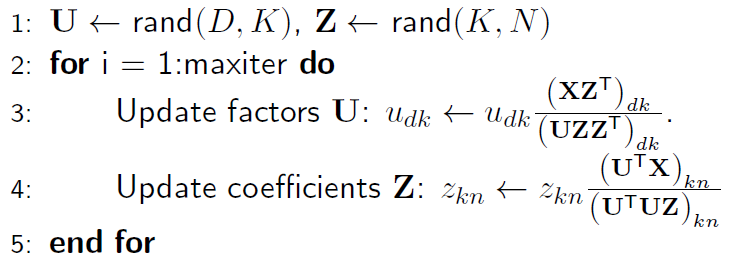
\includegraphics[width=0.9\linewidth]{nmf-quadratic}

If we allow negative entries in $U$ we get a {\bf semi-NMF} algorithm
iterating two steps:

\begin{enumerate}
    \item Data matrix $U$ is updated: 
    \begin{align*}
    U = XZ^\top (Z Z^\top)^{-1}
    \end{align*}
    \item Update $Z$:
    \begin{align*}
        z_{kn} \leftarrow z_{kn} \sqrt{
        \frac{
            (U^\top X)_{kn}^+ + \big[ (U^\top U)^- Z \big]_{kn}
        }{
            (U^\top X)_{kn}^- + \big[ (U^\top U)^+ Z \big]_{kn}
        }}
    \end{align*}
\end{enumerate}
With $a_{ij}^+ := \max(0, a_{ij}), a_{ij}^- := \min(0, a_{ij})$.\\
Equivalent to $K$-means if $Z$ is orthogonal.



\section{Sparse Coding}
Decompose original signal $z$ into orthonormal matrix $A$ and sparse signal
$\hat{x}$ by truncating small values in $x$ for $z = Ax$.

{\bf Overcompleteness} ($L > D$): more atoms (dictionary elements) than
dimensions. Therefore union of orthonormal bases $[U_1 \ldots U_B]$ form new $U
\in \R^{D \times (B\cdot D)} \Rightarrow$ Overcompleteness factor $=
\frac{L}{D}$. Increases the linear dependency between atoms which is measured by
{\bf coherence}:
\begin{align*}
    m(U) = \max_{i,j: i \neq j} \big| u_i^\top u_j \big|
\end{align*}
which is $0$ for orthogonal basis $B$ and $\geq \frac{1}{\sqrt{D}}$ if atom $u$
is added to $B$.

\subsection{Matching Pursuit (MP) Algorithm}
Minimize residual while selecting less than $K$ atoms from the dictionary:
\begin{align*}
    z^* = \argmin_z \| x - Uz \|_2 \quad \text{s.t.} \; \|z\|_0 \leq K
\end{align*}

{\bf MP-Algorithm:}
\begin{algorithmic}
\State $z\gets 0$, $r \gets z$
\Comment{Initialization}
\While{$\|z\|_0 < K$} \\
    \Comment{atom with maximum correlation to $r$}
    \State $d^* \gets \argmax_d |u_d^\top r|$ 
    \State $z_{d^*} \gets z_{d^*} + u_{u^*}^\top r$
    \Comment{update vector}
    \State $r \gets r - (u_{d^*}^\top r)u_{d^*}$
    \Comment{update residual}
\EndWhile
\end{algorithmic}

Exact recovery if $K < \frac{1}{2}\big( 1 + \frac{1}{m(U)}\big)$. If coherence
$m(U)$ small, explaining a generating atom with other atoms is not sparse.
Therefore, sparse coding recovers support.

\subsection{Sparse Coding for Inpainting}
Sparse coding on known parts of the image which allows predition of missing
parts by reconstruction from sparse code. Mask $M$ with $m_{d,d} = 1$ if pixel
$d$ is known and $0$ if missing.

\begin{align*}
    z^* =                &\min_z \|z\|_0 \\
    \text{s.t. } \quad   &\|M(x - Uz)\|_2 < \sigma
\end{align*}

Reconstruction: $\hat{x} = Mx + (I-M)Uz^*$

\subsection{Dictonary Learning}
\begin{enumerate}
    \item Coding: $Z^{t+1} \in \argmin_z \| X - U^t \cdot Z \|_F^2$
    \item Update: $U^{t+1} \in \argmin_U \|X - U \cdot Z^{t+1}\|_F^2$
\end{enumerate}

\section{Robust PCA}
Additive decomposition; minimize $rank(L) + \lambda \cdot card(S)$ \\
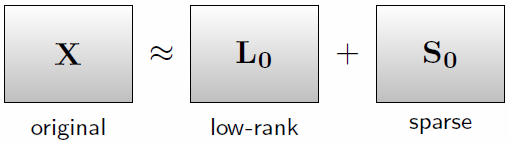
\includegraphics[width=0.9\linewidth]{rpca}

Convex Relaxation ($\|\cdot\|_*$ nuclear norm; $\|\cdot\|_1$: sum of all
absolute values):
\begin{align*}
    \text{minimize} \quad   & \|L\|_* + \lambda \|S\|_1 \\
    \text{subject to} \quad & L + S = X
\end{align*}

\subsection{Convexity}
A set $C$ is convex if the line segment between any two points in $C$ lies in
$C$. Function:
\begin{align*}
    f \text{ is convex } :\Leftrightarrow \quad &\forall x,y \in dom f, 0
    \leq \theta \leq 1: \\
    f( \theta x + (1 - \theta) y) & \leq \theta f(x) + (1 - \theta) f(y)
\end{align*}

{\bf Convex Optimization}: minimize $f(x)$ s.t. $g_i(x) \leq 0, h_i(x) = 0$
with $f(x)$ convex objective function, $g_i(x)$ inequality constraint functions,
$h_i(x)$ affine equality contrsint functions ($h_i(x) = a_i^\top x - b_i$)

{\bf Dual Problem}:
maximize $d(\lambda, \nu)$ s.t.
$\lambda \geq 0$, (Lagrangian, Lagrange dual function)
\begin{align*}
L(x, \lambda, \nu) 
&= f(x) + \sum_{i=1}^{m} \lambda_i g_i(x) + \sum_{i=1}^p \nu_i h_i(x) \\
d(\lambda, \nu) &= \inf_x L(x, \lambda, \nu)
\end{align*}

{\bf Dual Decomposition}:
\begin{algorithmic}
 \State $x_i^{k+1} := \argmin_{x_i} L_i(x_i, \nu^k), \quad \forall i$
 \State $\nu^{k+1} := \nu^k + \alpha^k \Big(\sum_{i=i}^N A_i x_i^{k+1} - b \Big)$
\end{algorithmic}


{\bf Alternating Direction Method of Multipliers (ADMM)} Minimize $f(x) + p(z)
s.t.
Ax + Bz = c$

\begin{algorithmic}
    \State $x^{k+1}$     := $\argmin_x L_\rho \big(x, z^k, \nu^k \big)$
    \State $z^{k+1}$     := $\argmin_z L_\rho \big(x^{k+1}, z, \nu^k \big)$
    \State $\nu^{k+1}$   := $\nu^k + \rho \big(Ax^{k+1} + Bz^{k+1} - c \big)$
\end{algorithmic}

{\bf Robust PCA} Solved with Principal Component Pursuit (PCP). Exact recovery
with probability $1 - \O(n^{-10})$, PCP with $\lambda = \frac{1}{\sqrt{N}}$ is
exact. $L_0$ of rank $\leq \rho_r n\mu^{-1} (\log n) ^{-2}$ and $S_0$ of
cardinality $m \leq \rho_s n^2$ ($\rho_s, \rho_r$ const.)

\clearpage
\end{multicols}
\end{document}
